\documentclass[10pt,dvipsnames,final]{beamer}
\usetheme{Copenhagen}
\usepackage[utf8]{inputenc}
\usepackage[french]{babel}
\usepackage[T1]{fontenc}
\usepackage{amsmath}
\usepackage{amsfonts}
\usepackage{amssymb}
\usepackage{graphicx}

%\setbeamercolor{titlelike}{parent=structure,fg=yellow,bg=violet}

\usepackage{listings}

\lstdefinelanguage{pdl}{
  keywords={Si, ALORS, Sinon, finSi, Pour, allant de,  FAIRE, finPour, tantQue, finTantQue, fonction, finFonction, action, finAction, Struct, finStruct, dansLeCasDe, case, default},
  keywordstyle=\color{RedOrange}\bfseries,
  keywords=[2]{booleen, chaine, entier, reel, caractere},
  keywordstyle=[2]\color{NavyBlue}\bfseries,
  keywords=[3]{retourner, constante},
  keywordstyle=[3]\color{Plum}\bfseries,
  identifierstyle=\color{black},
  sensitive=false,
  comment=[l]{//},
  morecomment=[s]{/*}{*/},
  commentstyle=\color{Gray}\ttfamily,
  stringstyle=\color{ForestGreen}\ttfamily,
  morestring=[b]',
  morestring=[b]"
}

\lstset{
   language=pdl,
   extendedchars=true,
   basicstyle=\footnotesize\ttfamily,
   showstringspaces=false,
   showspaces=false,
   tabsize=3,
   breaklines=true,
   showtabs=false
}


\title{Analyse Puyo Puyo et Super off road}
\author{Rachel~\textsc{Humbert} \and Emma~\textsc{Mange} \and Alphée~\textsc{Grosdidier} \and Anton~\textsc{Dolard} \and Silvio~\textsc{Vescovo}}

\logo{\includegraphics[width=1cm]{reseauFigure}\includegraphics[width=1cm]{nom_universite}}
\institute[UFC]{Université de Franche-Comté}
\date{2020 -- 2021}


\newcommand{\midcolumn}[2]{
\begin{columns}
	\begin{column}{0.5\textwidth}
		#1
	\end{column}
	\begin{column}{0.5\textwidth}
		#2
	\end{column}
\end{columns}
}


\setbeamertemplate{footline}
{
  \leavevmode%
  \hbox{%
  \begin{beamercolorbox}[wd=.63\paperwidth,ht=2.25ex,dp=1ex,center]{author in head/foot}%
    \usebeamerfont{author in head/foot}\insertshortauthor
  \end{beamercolorbox}%
  \begin{beamercolorbox}[wd=.37\paperwidth,ht=2.25ex,dp=1ex,center]{title in head/foot}%
    \usebeamerfont{title in head/foot}\insertshorttitle\hspace*{1em}
    \insertframenumber/\inserttotalframenumber\hspace*{1ex}
  \end{beamercolorbox}}%
  \vskip0pt%
}

\begin{document}


\AtBeginSection{%
  \begin{frame}
    \tableofcontents[sectionstyle=show/shaded,subsectionstyle=hide,subsubsectionstyle=hide]
  \end{frame}
}

\AtBeginSubsection[]
{
\begin{frame}{Plan}
\tableofcontents[sectionstyle=show/hide,subsectionstyle=show/shaded/hide,subsubsectionstyle=show/shaded/shaded/hide]
\end{frame}
}

\AtBeginSubsubsection[]
{
\begin{frame}{Plan}
\tableofcontents[sectionstyle=show/hide,subsectionstyle=show/shaded/hide,subsubsectionstyle=show/shaded/shaded/hide]
\end{frame}
}

\begin{frame}
\titlepage
\end{frame}

\section{Puyo Puyo}

\subsection{Présentation du jeu}

\begin{frame}
\midcolumn{\includegraphics[width=\textwidth]{presentationfiles/Sega-Ages-Puyo-Puyo_03-24-19}}{
\begin{itemize}
	\item Jeu de type Puzzle
	\item Développé par \emph{Compile}
	\item Sorti en 1991
\end{itemize}
}
\end{frame}

\subsection{État du jeu}

\begin{frame}{Les structures et variables}
\begin{itemize}
\item Les variables du jeu
\begin{itemize}
\item constante entier NBCOLORS 
\item constante entier HEIGHT
\item constante entier WIDTH
\item constante entier FALLSPEED 
\item constante entier SIZEPUYO
\item constante entier WIDTHMAT
\item constante entier HEIGHTMAT
\item constante entier WAITINGPOSX
\item constante entier WAITINGPOSY
\item booleen doStartTour
\item booleen gameOver
\item entier penaltyReps1
\item entier penaltyReps2
\end{itemize}
\end{itemize}
\end{frame}

\begin{frame}{Les structures et variables}
\begin{itemize}
\item Structures générales (qui ne représentent pas un objet du jeu)
\begin{itemize}
\item structure Position
\end{itemize}
\item Structures qui représentent un élément du jeu
\begin{itemize}
\item structure Block
\item structure BlockFall
\item structure Player
\item structure Game
\end{itemize}
\end{itemize}
\end{frame}

\begin{frame}{Block \& BlockFall}
\midcolumn{\lstinputlisting[language=pdl]{pdl/puyopuyo/Block.txt}}{\includegraphics[width=\textwidth]{presentationfiles/block-img}}
\end{frame}

\begin{frame}{BlockFall}
\midcolumn{\lstinputlisting[language=pdl]{pdl/puyopuyo/BlockFall.txt}}{\includegraphics[width=\textwidth]{presentationfiles/BlockFall}}
\end{frame}

\begin{frame}{Player \& Game}
\midcolumn{\lstinputlisting[language=pdl]{pdl/puyopuyo/Player.txt}}{\lstinputlisting[language=pdl]{pdl/puyopuyo/Game.txt}}
\end{frame}

\subsection{Configuration initiale du jeu}

\begin{frame}{État initial}
\includegraphics[width=\textwidth]{presentationfiles/Capture_decran_2021-03-21_a_21.51.47} 
\end{frame}

\subsection{Évolution du jeu}

\subsubsection{Action du joueur}

\begin{frame}{Pression sur L ou R}
\lstinputlisting[language=pdl]{pdl/puyopuyo/leftMotion.txt}
\end{frame}

\begin{frame}{La touche D}
\begin{block}{Pression sur D}
\lstinputlisting[language=pdl]{pdl/puyopuyo/downMotion.txt}
\end{block}
\begin{block}{Relachement de D}
\lstinputlisting[language=pdl]{pdl/puyopuyo/stopDownMotion.txt}
\end{block}
\end{frame}

\begin{frame}{Appui sur une flèche directionnelle}
Pour la flèche gauche:
\lstinputlisting[language=pdl]{pdl/puyopuyo/leftOrient.txt}
On fera de même pour la flèche haut, droite et bas. Nous attribuerons respectivement à p1.bf1.orient 1, 2 ou 3, et modifieront les conditions de manière à ce qu'elles correspondent à chaque direction.
\end{frame}

\subsubsection{Règles du jeu}

\begin{frame}[allowframebreaks]{Boucle Principale}
\lstinputlisting[language=pdl]{pdl/puyopuyo/boucleJeu.txt}
\end{frame}

\subsection{Algorithmes}

\begin{frame}{continueFall}
\lstinputlisting[language=pdl]{presentationfiles/continueFallDiapo.txt}
\end{frame}

\begin{frame}{blockDown}
\lstinputlisting[language=pdl]{presentationfiles/blockDownDiapo.txt}
\end{frame}

\begin{frame}[allowframebreaks]{AttribuerGroupe}
\lstinputlisting[language=pdl]{pdl/puyopuyo/AttribuerGroupe.txt}
\end{frame}

\begin{frame}{resetBlocksForID}
\lstinputlisting[language=pdl]{presentationfiles/resetBlockForIDDiapo.txt}
\end{frame}

\begin{frame}{destroyBlock}
\lstinputlisting[language=pdl]{pdl/puyopuyo/destroyBlock.txt}
\end{frame}

\begin{frame}{setClearBlocksOnPlayer}
\lstinputlisting[language=pdl]{pdl/puyopuyo/setClearBlocksOnPlayer.txt}
\end{frame}

\section{Super off road}

\subsection{Présentation du jeu}

\begin{frame}
\midcolumn{\includegraphics[width=\textwidth]{presentationfiles/super_off_road_us_box_art}}{
\begin{itemize}
	\item Jeu de course
	\item Développé par Leland Corporation
	\item Sorti en 1989 sur borne d'arcade
\end{itemize}
}
\end{frame}

\subsection{État du jeu}

\begin{frame}{Les structures et variables}
\begin{itemize}
\item Variables générales du jeu
\begin{itemize}
\item constante entier ACCELERATION
\item constante entier NB\_LAPS
\item constante entier NITRO\_TIME
\item constante entier NITRO\_WIDTH
\item constante entier NITRO\_SPAWN\_TIME
\item constante entier CAR\_WIDTH
\item constante entier CAR\_HEIGHT
\item Car playerCar
\item Bonus [] nitroList
\item entier malusBonusSpeed <- 1
\end{itemize}
\end{itemize}
\end{frame}


\begin{frame}{Les structures et variables}
\begin{itemize}
\item Structures générales (qui ne représentent pas un objet du jeu)
\begin{itemize}
\item structure Position
\item structure Hitbox2P
\item structure Hitbox4P
\item structure Speed
\end{itemize}
\item Structures qui représentent un élément du jeu
\begin{itemize}
\item stucture Flag
\item structure Wall
\item structure Car
\item structure Bonus
\item structure Mud
\item Structure Ground
\end{itemize}
\end{itemize}
\end{frame}

\begin{frame}{Hitbox2P et Hitbox4P}
\lstinputlisting[language=pdl]{pdl/superOffRoad/Hitbox2P.txt}
\lstinputlisting[language=pdl]{pdl/superOffRoad/Hitbox4P.txt}
\end{frame}

\begin{frame}{Flag \& Wall}
\midcolumn{\lstinputlisting[language=pdl]{pdl/superOffRoad/Flag.txt}\lstinputlisting[language=pdl]{pdl/superOffRoad/Wall.txt}}{\includegraphics[width=\textwidth]{presentationfiles/flags-walls-sor}}
\end{frame}

\begin{frame}{Car \& Bonus}
\midcolumn{\lstinputlisting[language=pdl]{pdl/superOffRoad/Car.txt}\lstinputlisting[language=pdl]{pdl/superOffRoad/Bonus.txt}}{\includegraphics[width=\textwidth]{presentationfiles/cars-bonus-sor}}
\end{frame}

\begin{frame}{Mud \& Ground}
\midcolumn{\lstinputlisting[language=pdl]{pdl/superOffRoad/Mud.txt}\lstinputlisting[language=pdl]{pdl/superOffRoad/Ground.txt}}{\includegraphics[width=\textwidth]{presentationfiles/Mud}}
\end{frame}

\subsection{Configuration initiale du jeu}

\begin{frame}{État initial}
\includegraphics[width=\textwidth]{presentationfiles/initial-state-sof} 
\end{frame}

\subsection{Évolution du jeu}

\subsubsection{Action du joueur}

\begin{frame}{Actions utilisateurs}
\lstinputlisting[language=pdl]{presentationfiles/ActionUtilisateur.txt}

On fait de même avec les touches q, s, d et spacebar où l'on change respectivement les valeurs de \emph{gauche}, \emph{bas},\emph{droite} et \emph{nitro}.

\lstinputlisting[language=pdl]{presentationfiles/TournerUtilisateur.txt}
\end{frame}

\subsubsection{Règles du jeu}

\begin{frame}{Condition de victoire}
\midcolumn{Le joueur gagne lorsqu'il est le premier à effectuer les 3 tours de circuit dans le sens imposé. Pour cela, il peut utiliser de l'argent avant la course pour s'acheter des améliorations, et peut aussi utiliser les boosts disponibles sur le terrain durant la course.}{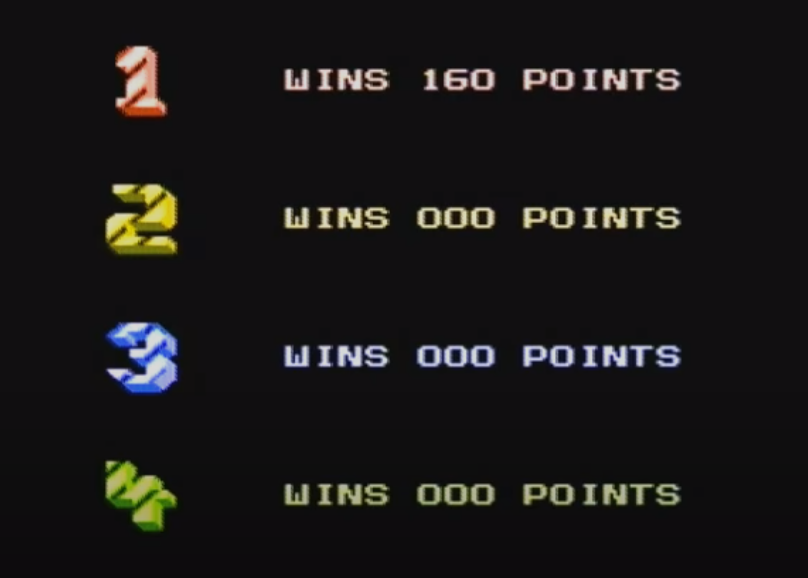
\includegraphics[width=\textwidth]{presentationfiles/fin_partie}} 
\end{frame}

\subsection{Algorithmes}

\begin{frame}[fragile]{calculateSpeed}
\begin{lstlisting}[language=pdl]
fonction Speed calculateSpeed ( -> Car car , -> entier acceleration , -> entier avgAcceleration , -> booleen isAccelerate , -> booleen isBreack , -> booleen isNitro, -> reel dt )
\end{lstlisting}

On calcule la nouvelle vitesse de la voiture en fonction de son accélération (qui dépendra des obstacles) ainsi que des actions de l'utilisateur.
\end{frame}

\begin{frame}{isCollision}
\lstinputlisting[language=pdl]{pdl/superOffRoad/isColision.txt}
\end{frame}

\begin{frame}{countTour}
\lstinputlisting[language=pdl]{pdl/superOffRoad/countTour.txt}
\end{frame}

\begin{frame}{spawnNitro}
\lstinputlisting[language=pdl]{pdl/superOffRoad/generateNitro.txt}
\end{frame}

\begin{frame}{Conclusion}
\Huge\centering
Des questions ?
\end{frame}

\end{document}
